% Template file for an LPSC Poster
% Written by Moses P. Milazzo
% Copyright (C) 2008, 2009, 2010, 2011, 2012, 2014
%
% This work is licensed under the Creative Commons
% Attribution-Noncommercial-Share Alike 3.0 License. To view a copy
% of this license, visit http://creativecommons.org/licenses/by-nc-sa/3.0/;
% or, (b) send a letter to Creative Commons, 171 2nd Street, Suite
% 300, San Francisco, California, 94105, USA.

\documentclass[lpsc]{lpscposter}
% You might find the 'draft' option useful if you have
% lots of graphics, because they can take some time to process and
% display. (\documentclass[draft]{lpscposter}) However, you'll
% see no images if you do this, just placeholders.

\pagestyle{empty}
\setcounter{secnumdepth}{0}

% The textpos package is necessary to position textblocks at arbitary 
% places on the page.
\usepackage[absolute]{textpos}

% Use numbers as references, just like the LPSC abstract.
\usepackage[numbers]{natbib}

% Use the Times package for a Times typeface. Other typefaces are also available.
%\usepackage{Times}

% Arial typeface
%\usepackage[scaled]{uarial}
%\renewcommand*\familydefault{\sfdefault} %% Only if the base font of the document is to be sans serif
%\usepackage[T1]{fontenc}

% Helvetica typeface
\usepackage[scaled]{helvet}
\renewcommand*\familydefault{\sfdefault} %% Only if the base font of the document is to be sans serif
\usepackage[T1]{fontenc}

% Use the underscore package to make underscores look good.
%\usepackage{underscore}

% You probably don't need all of these graphics packages,
% so remove the ones that don't have anything to do with your particular
% input graphics.
\usepackage{graphics,wrapfig}
\usepackage{eso-pic,graphicx,paralist}

% These colours are tried and tested for titles and headers. Don't
% over use color!
\usepackage{color}
\definecolor{DarkBlue}{rgb}{0.1,0.1,0.5}
\definecolor{Red}{rgb}{0.9,0.0,0.1}
\definecolor{Orange}{rgb}{0.8,0.5,0.0}
\definecolor{Green}{rgb}{0.0,0.44313,0.31373}

% If you want to put color in the background of textblocks, define the colors you want
% to use. Don't over-do this or your poster will look awful.
% \definecolor{MyTextBlockColor}{rgb}{1,0.9,0.6}
% Within the poster, you'll define textblock colors as follows:
% \textblockcolor{MyTextBlockColor}
% Every textblock following will have this color.

\usepackage{ragged2e}

% Set up the text header sizes for this particular poster.
\let\Textsize\small
\def\Head#1{\noindent\hbox to \hsize{\hfil{\LARGE\color{Green} #1}}\bigskip}
\def\RHead#1{\noindent\hbox to \hsize{\hfil{\LARGE\color{Green} #1|}}}
\def\leftHead#1{\hbox to \hsize{{\LARGE\color{Green} #1}}}
\def\LHead#1{\noindent{\LARGE\color{Green} #1}\bigskip}
\def\Lhead#1{\noindent{\Large\color{Green} #1}\bigskip}
\def\Subhead#1{\noindent{\large\color{Green} #1}\bigskip}
\def\Title#1{\noindent{\VERYHuge\color{Green} #1}}

\renewcommand\refname{}


% Set up the grid
%
% Note that [40mm,40mm] is the margin round the edge of the page.
% The grid size is given by the {23}{23} options.
% This poster is square at 42 inches. \textpos is not terribly
% clear on how to be specific about overall page size.
\TPGrid[40mm,40mm]{23}{23}      % 3 cols of width 7, plus 2 gaps width 1

% Set a small margin around the textbox frame. This will be the default
% even if we're not showing the frame so that all textboxes have the
% same margins.
\TPMargin{0.5em}

% Set up some paragraph controls.
\parindent=0pt
\parskip=0.5\baselineskip


% These packages are for the nonsense text filler
\usepackage[english]{babel}
\usepackage{blindtext}


\begin{document}
% Understanding textblocks is the key to being able to do a poster in
% LaTeX. In
%
%    \begin{textblock}{wid}(x,y)
%    ...
%    \end{textblock}
%
% the first argument gives the block width in units of the grid
% cells specified above in \TPGrid; the second gives the (x,y)
% position on the grid, with the y axis pointing down.

% You will have to do a lot of previewing to get everything in the 
% perfect place.

% This gives good title positioning for a portrait poster.
% Watch out for hyphenation in titles - LaTeX will do it
% but it looks awful.
\begin{textblock}{21}(1,0)
  \begin{center}
    \Title{M.P. Milazzo's LPSC \LaTeX\ Poster Template}
  \end{center}
\end{textblock}

% This puts a small textblock on the right-hand side upper corner to
% allow passers-by to look up the abstract number and authors and
% their affiliations.
\begin{textblock}{3}(20.25,0)
  Abstract 12345\\
  {\footnotesize $^{*}$M.P. Milazzo, OtherOrb Science, Flagstaff, AZ}
\end{textblock}

% OtherOrb Logo; replace with your institution logo if you like.
% This logo appears in the upper left corner of the poster. 
\begin{textblock}{3}(0,0)
  
\includegraphics[width=0.75\textwidth]{OtherOrbLogoGold.png}
\end{textblock}

% the {4.2}(0,1) indicates the size and position of the textblock. You'll want to 
% adjust these until things look good for your particular poster. When you find an
% arrangement you like, these will probably not change a lot from year-to-year.
\begin{textblock}{4.2}(0,1.2)
  \Head{Introduction}
  %\slshape
  \small
  This template is created to help those who use
  \LaTeX\ write LPSC posters that look decent, are output as
  scaleable PDFs, and can be printed by most modern large-format printers
  with little or no fiddling.
  
  We turned off paragraph indentation. 
  If you want it back on, look at the preamble and comment out the \verb=\parindent= command. 
  Also, you can do citations just like normal \cite{kopka2003guide}.
  
  Here is some nonsense text to fill in this box.
  \blindtext
  \bigskip
\end{textblock}

\begin{textblock}{4.2}(0,12.2)
  \Head{Left Section Header}
  %\slshape
  \small
  You use citations and references exactly as you would for any \LaTeX\ publication. 
  Here's our second and third citation \cite{light2004end,borland2007rainbow}. 
  And let's also cite \cite{green2011colour}.

\begin{table}
\caption{
\label{Col_Joints_Table}
  \small
 I would like to include a small table too. So let's do that:}
 \begin{center}
   \begin{tabular}{llll}
   \textbf{Column 1} & \textbf{Column 2} & \textbf{Column 3} & \textbf{Confidence}\\
   \hline
   Just & Like & Any & Other\\
   Table & We & Can & Format\\
   This & As & We & Like.\\
   This & As & We & Like.\\
   This & As & We & Like.\\
   This & As & We & Like.\\
   This & As & We & Like.\\
   \hline
  \end{tabular}
\end{center}
\end{table}
  
  \bigskip
\end{textblock}

% Note that the Section styles here and below are \LHead rather than 
% \Head. That's because these are on the right-hand-side of the poster and 
% the \LHead command left-justifies the headers while the \Head command
% right-justifies the headers. If you don't like this, modify the lpscposter style file
% to fit your needs.

\begin{textblock}{4.2}(19,1.2)
  \LHead{Right Section Header}
  %\slshape
  \small 
  
  Remember that you don't want to overwhelm your viewers with text. 
  Use a little bit of text to explain what you did, make the captions to your figures excessively helpful, and leave the rest for the conversation with people who come to your poster. 
  If you intend to be absent from your poster during the session, leave a copy or a URL for a copy of your abstract, paper, etc., so interested people can find out more about what you did.
  
  Whatever you do, don't ask your viewers to ingest tons of text all at once; they'll go elsewhere. 
  The poster session is as much about networking as it is about presenting your results. 
  Do both verbally.
\end{textblock}

% Turn on box frame for this one textblock.
\TPshowboxestrue
\begin{textblock}{4.2}(19,12.2)
  \LHead{Concluding Remarks}
  %\slshape
  \small
  
  For the most part, you'll be fiddling with textblock positions and sizes to make things
  perfect. 
  Unfortunately, until you've written your entire poster, you won't know exactly 
  where everything should fit or how large specific blocks should be. 
  You'll notice that the figures don't line up perfectly at the bottom but they do line up at the top. 
  If you want perfect alignment, you have to make your figures and their captions about the same size.
  
  Be careful with showing the frames around boxes; you might be surprised at where frame boxes
  start and stop and how they overlap.
  \bigskip
\end{textblock}

% The References section is just a textblock like all the others, but
% it contains the bibliography. This bibliography looks a lot like the LPSC
% abstract bibliography offered elsewhere by me because it's pretty much
% the same.

% Turn off the visible frame again.
\TPshowboxesfalse
\begin{textblock}{4.2}(19,15.5)
  \Lhead{References}
  \slshape
  \small
  \begin{inparaenum}
    \bibliographystyle{lpscposter}
    \fussy
    % Hide the default references title in place of the header I set above. I like the 
    % text color of the section headers to be the same, including for the References section.
     \renewcommand{\section}[2]{}
      \raggedright
      \bibliography{templatebibliography.bib}
  \end{inparaenum}
\end{textblock}


% Figures, in order of their reference within the document if you're using "Figure 1" notation.
% Note that this is not necessarily the same order as the appear left->right top->down on the
% poster unless you want it to be. Sometimes larger figures fit better in certain places even if
% that makes them appear to be out of place. Just be clear so your reader doesn't have to
% fight your poster to get information from it...
% I place the figures last in the LaTeX document because it's just easier for me to keep track 
% of where they are. It doesn't really matter, though, because we're not allowing them to float 
% as one would in a normal LaTeX document.


% Figure 1
\begin{textblock}{7}(4.5,1.2)
	\begin{center}
	\begin{figure}
	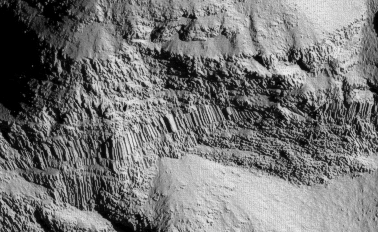
\includegraphics[width=\textwidth]{PSP_006985_2020_RED_NOMAP_crop2012_2}
		\caption{
		\scriptsize
		{\em One column wide figure}
		\label{MartianColumns}
		}
	\end{figure}
	\end{center}
\end{textblock}

% Figure 2; Spans the entire poster, so it has a large textblock size (23.1). Its x-position is 0, and its y-position
% is appropriate for where it appears on the poster.
\begin{textblock}{23.1}(0,5.9)
\begin{figure}
\begin{center}
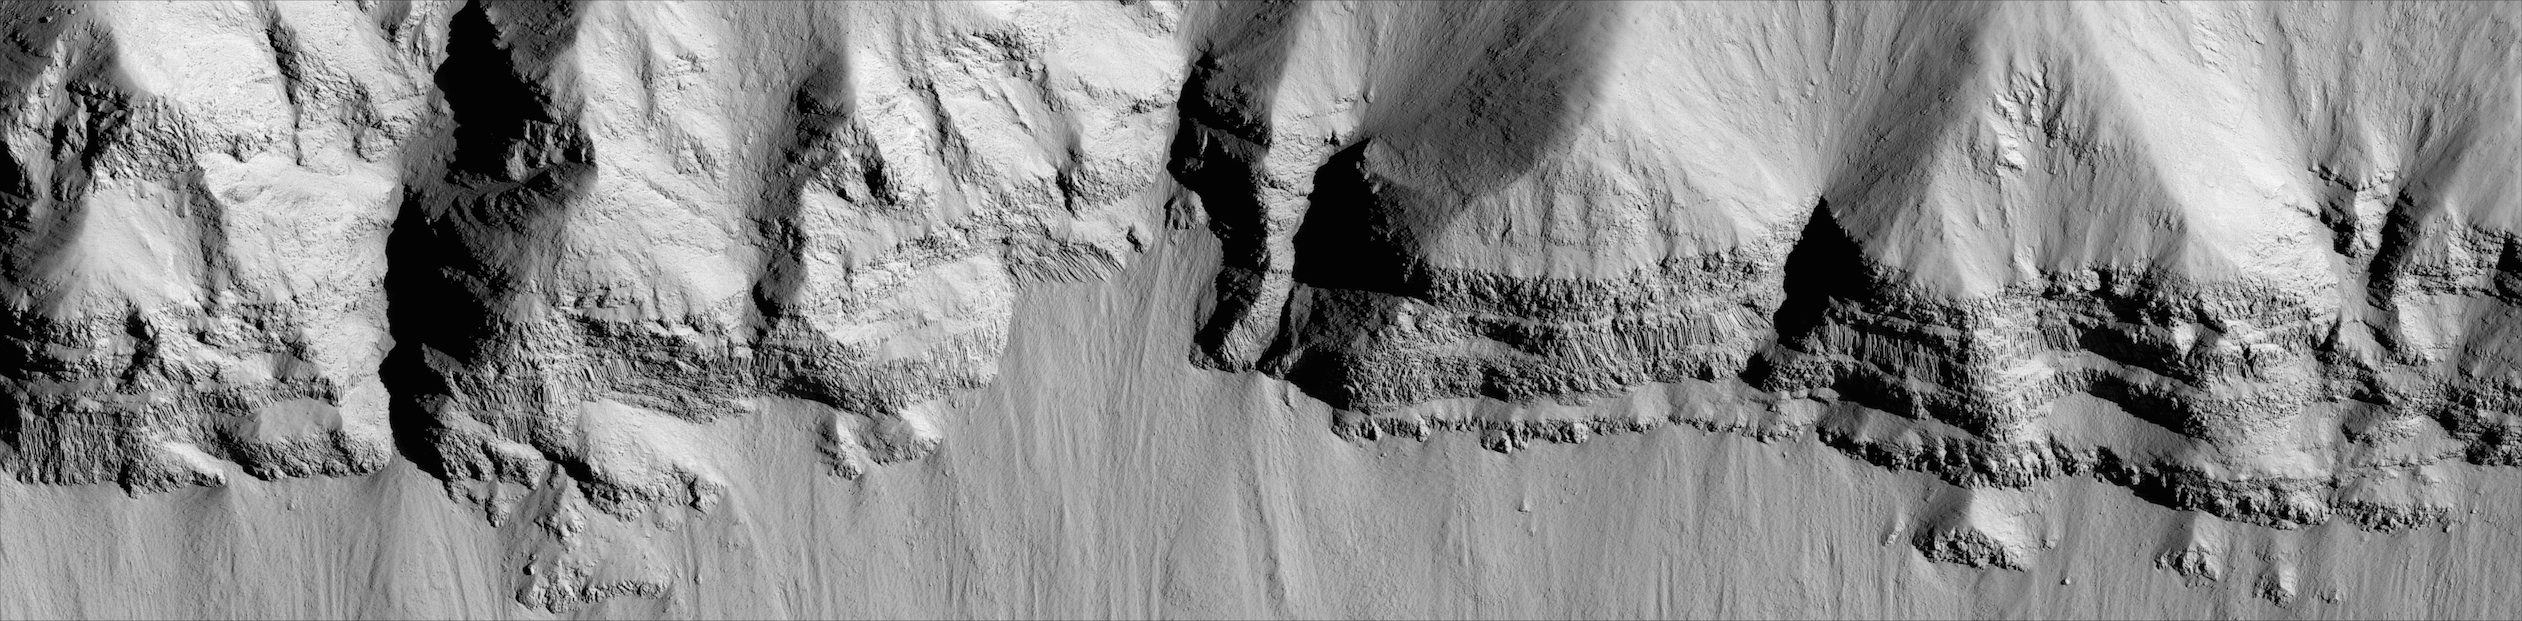
\includegraphics[width=\textwidth]{PSP_006985_2020_RED_NOMAP_2172009_31759}
	\caption{
	\scriptsize
	{\em This figure is a multi-column (three columns wide) figure, so I made its textblock wide (23.1 units).}
	\label{MartianColumns2}
	}
\end{center}
\end{figure}
\end{textblock}

% Figure 3. I like having my figures in the center of the poster but you can move them wherever you like.
\begin{textblock}{7}(11.75,1.2)
\begin{center}
\begin{figure}
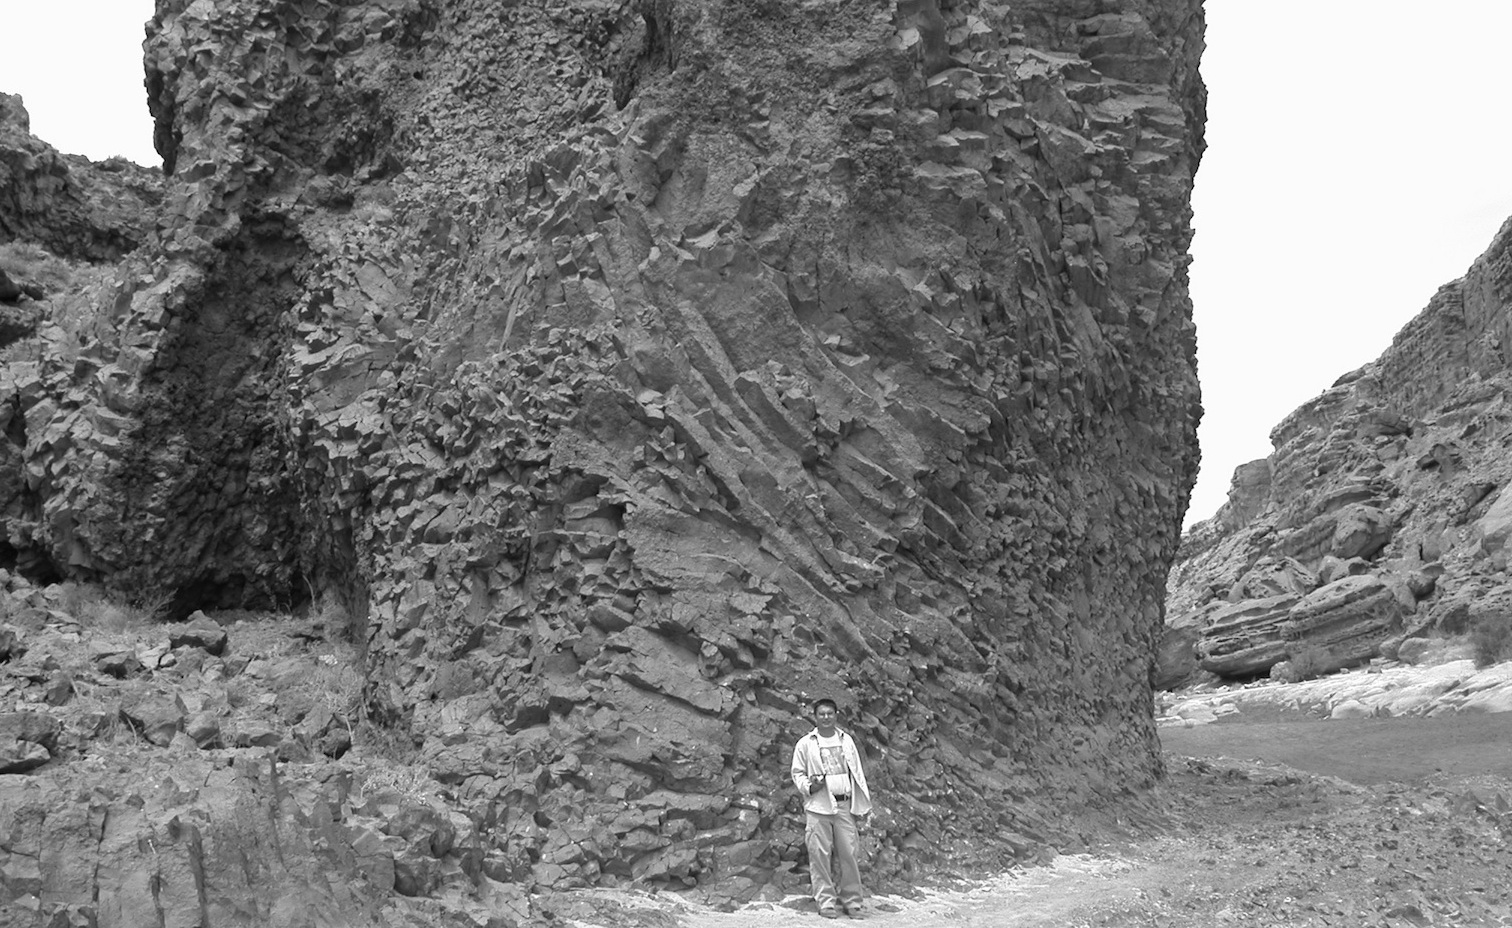
\includegraphics[width=\textwidth]{Milazzo_Columnar_Jointing_grand_falls_grey_crop}
	\caption{
	\scriptsize
	{\em Entablature at Grand Falls, Arizona with the standard Laz Kestay unit for scale.}
	\label{GrandFalls}
	}
\end{figure}
\end{center}
\end{textblock}


\begin{textblock}{7}(4.5,12.75)
\begin{figure}
	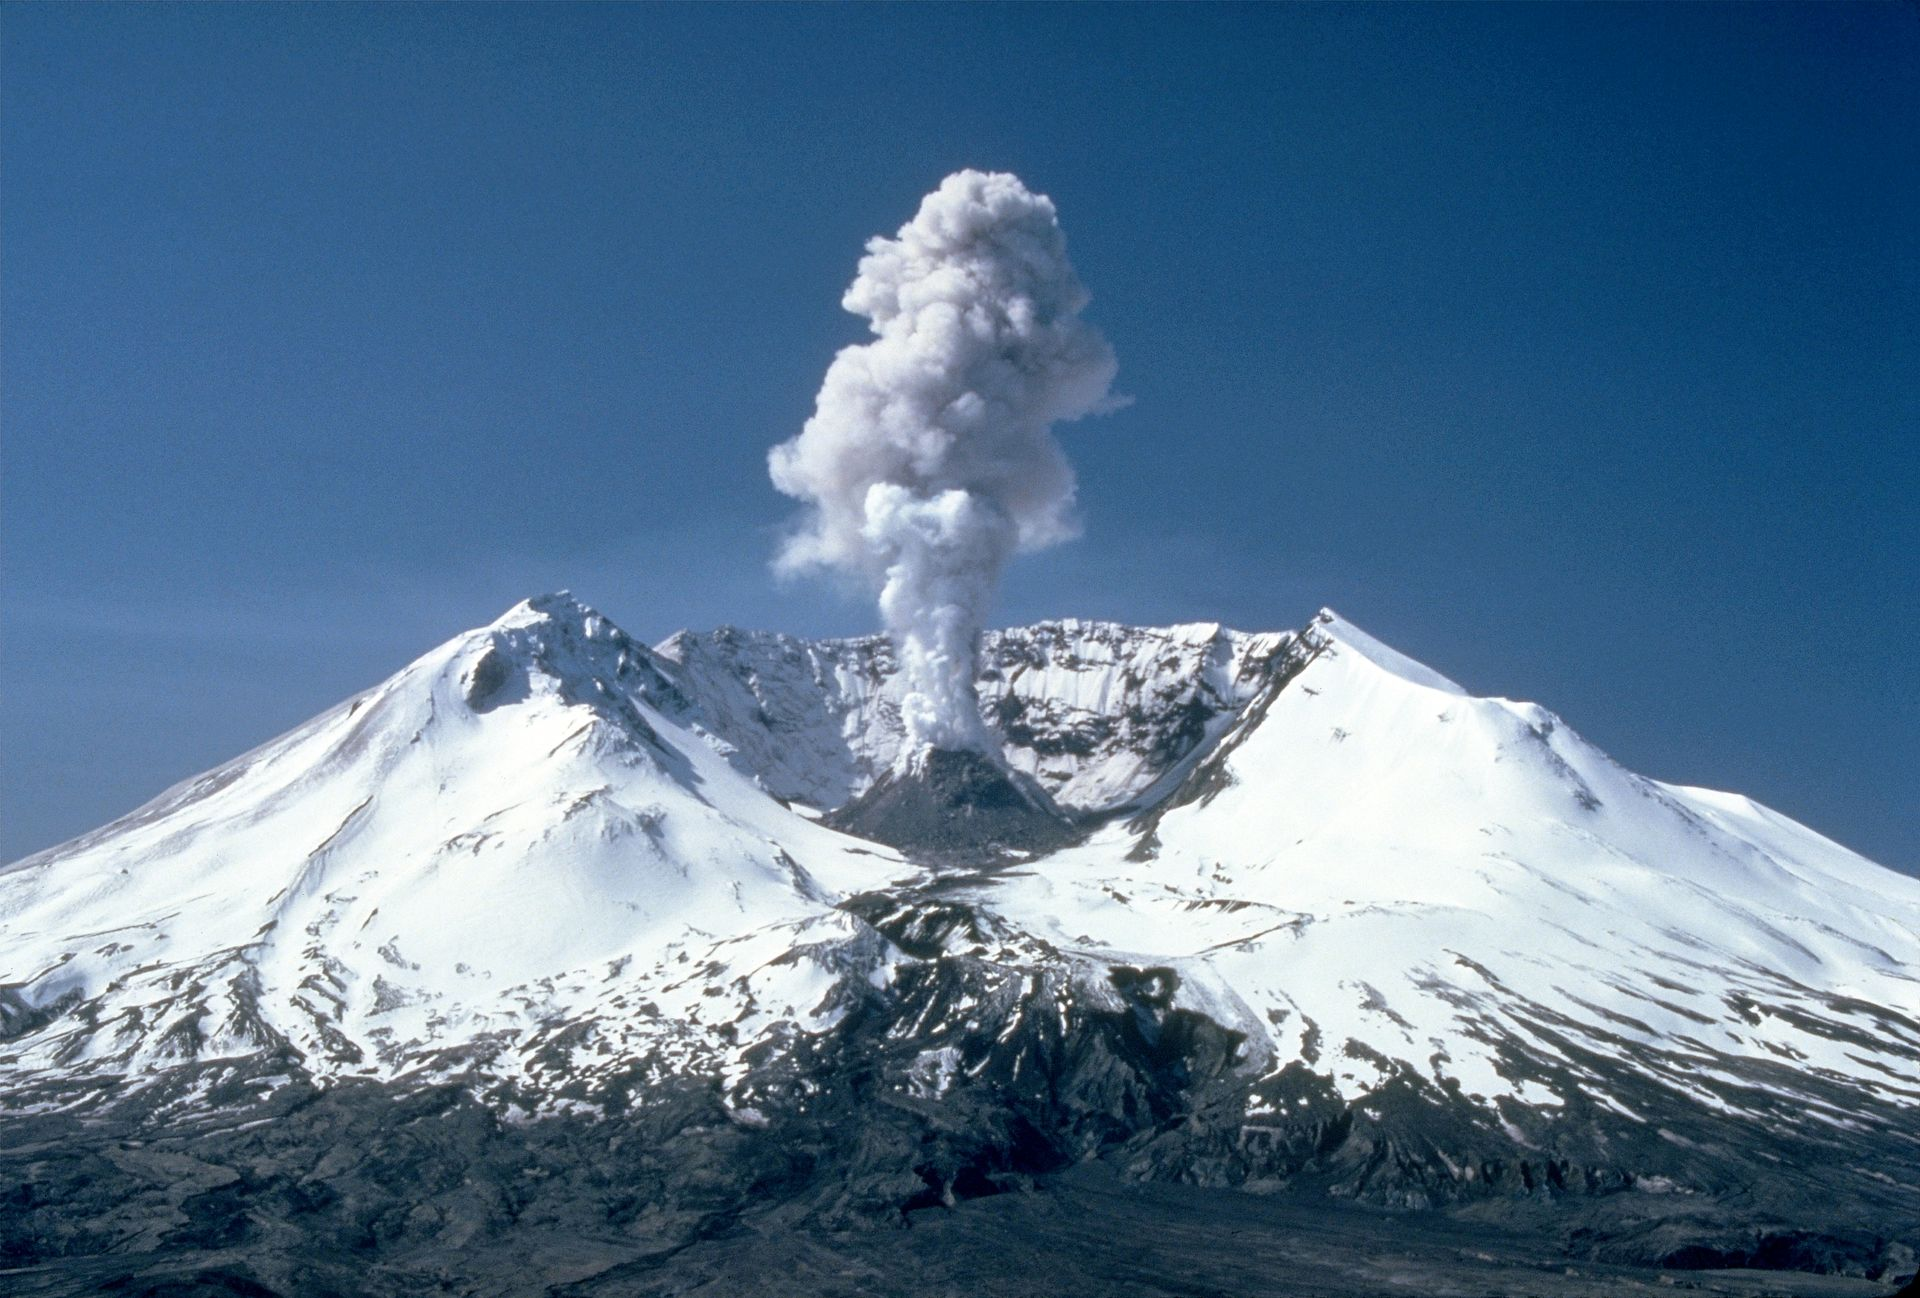
\includegraphics[width=\textwidth]{MSH_1982}
	\caption{
	\scriptsize
	{\em Mount St. Helens taking a break.}
	\label{msh}
	}
\end{figure}
\end{textblock}


\begin{textblock}{7}(11.75,12)
\begin{figure}
	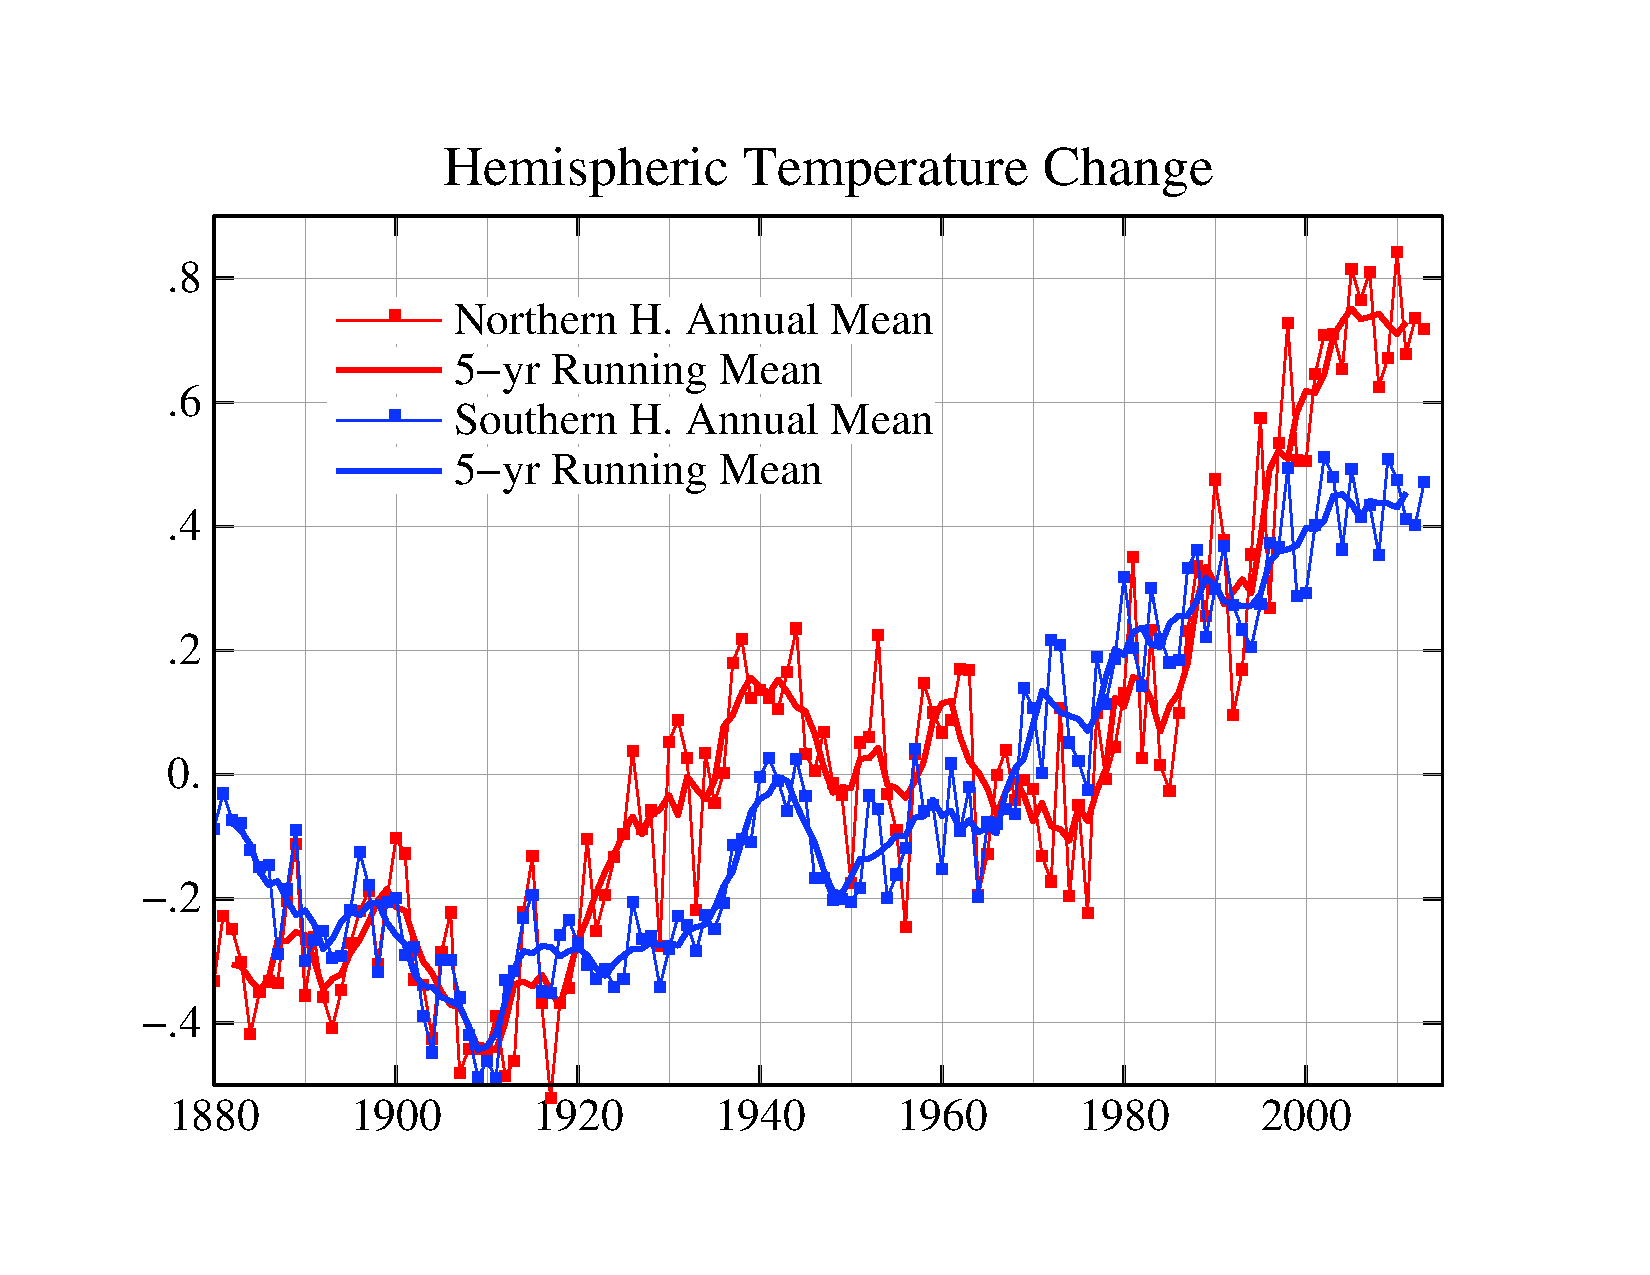
\includegraphics[width=\textwidth]{FigA3.pdf}
	\caption{
	\scriptsize
	{\em Higher and higher.}
	\label{hot}
	}
\end{figure}
\end{textblock}


\begin{textblock}{7}(0,18)
\begin{center}
\begin{figure}
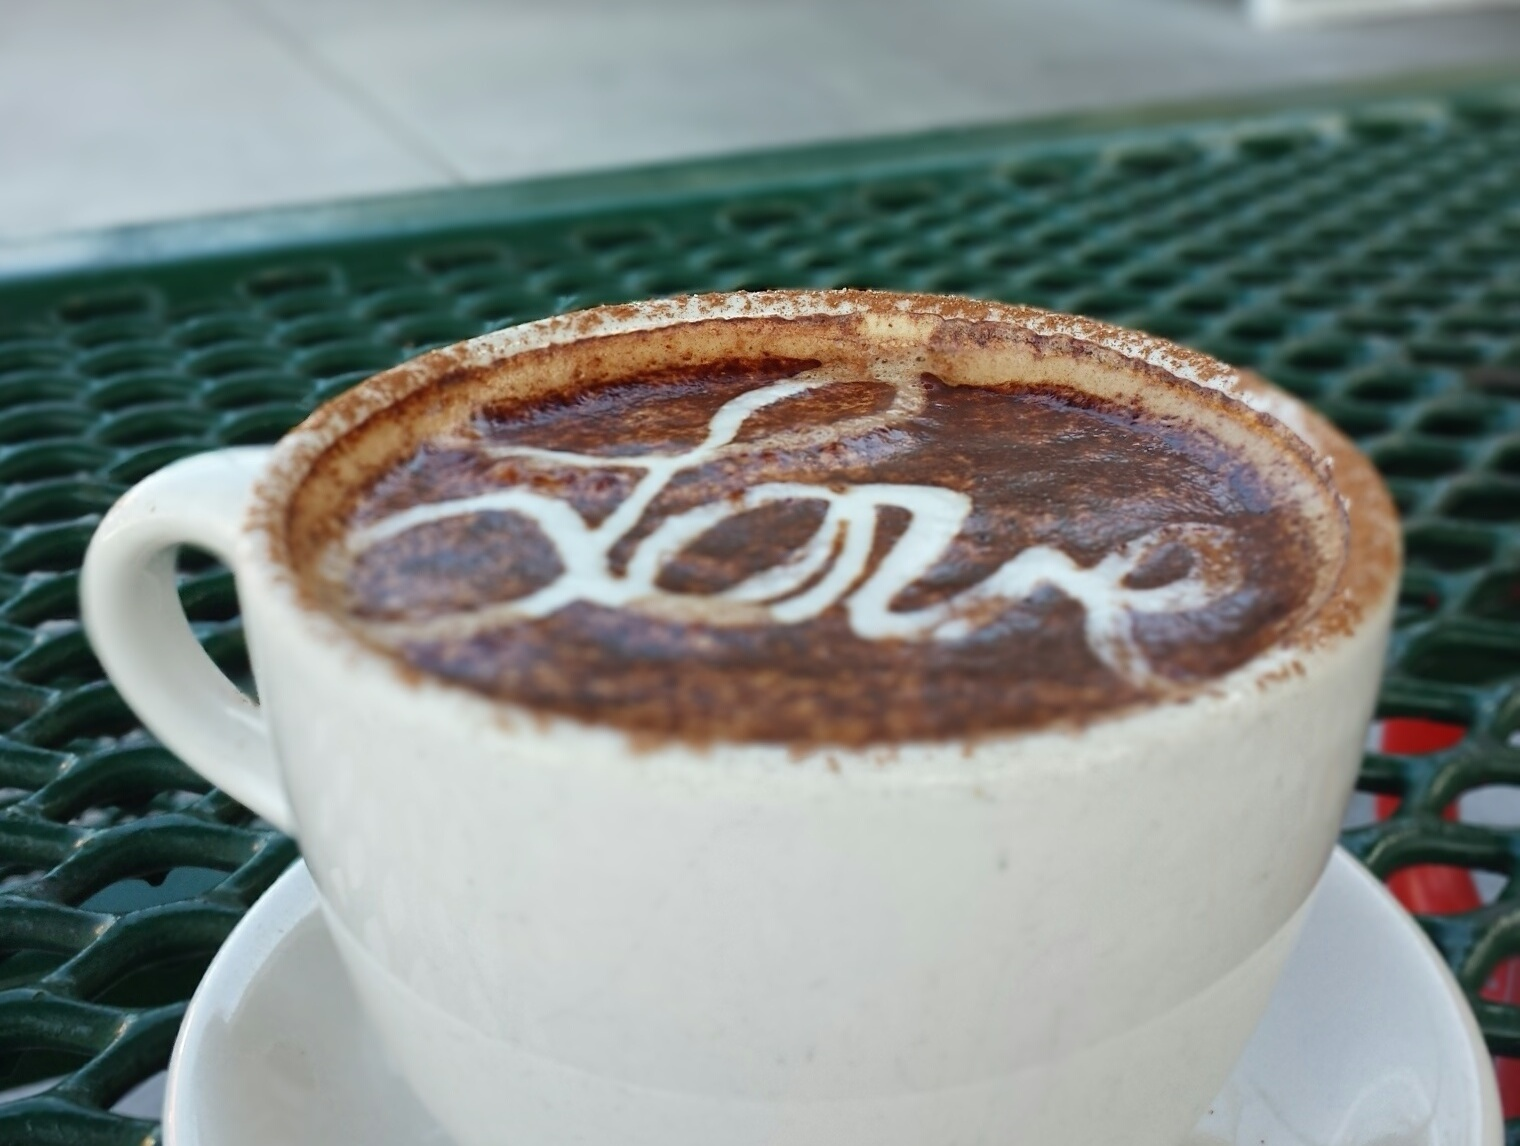
\includegraphics[width=\textwidth]{Coffee}
	\caption{
	\scriptsize
	{\em I do love my coffee \dots You can add figure captions as normal, of course}
	\label{Utah}
	}
\end{figure}
\end{center}
\end{textblock}

\begin{textblock}{7}(8,18)
\begin{center}
\begin{figure}
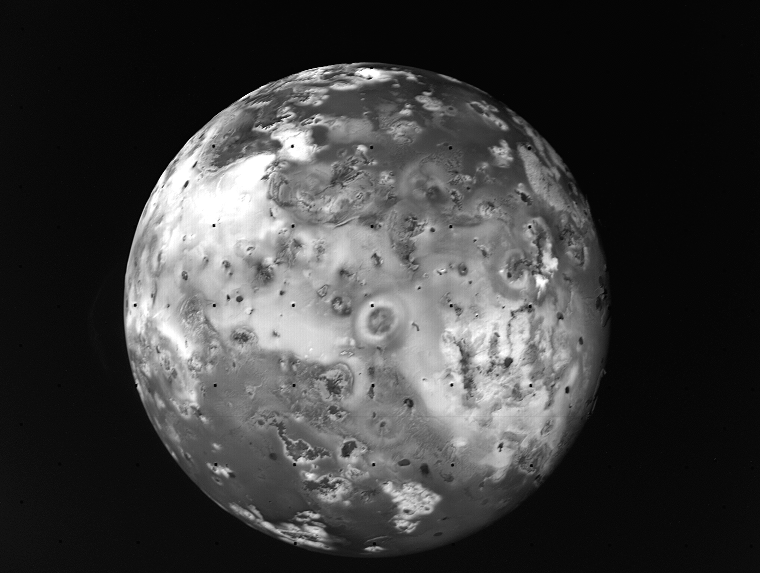
\includegraphics[width=\textwidth]{vg1_Io}
	\caption{
	\scriptsize
	{\em Voyager 1 image of Io}
	\label{vg1io}
	}
\end{figure}
\end{center}
\end{textblock}


\begin{textblock}{7}(16,18)
\begin{center}
\begin{figure}
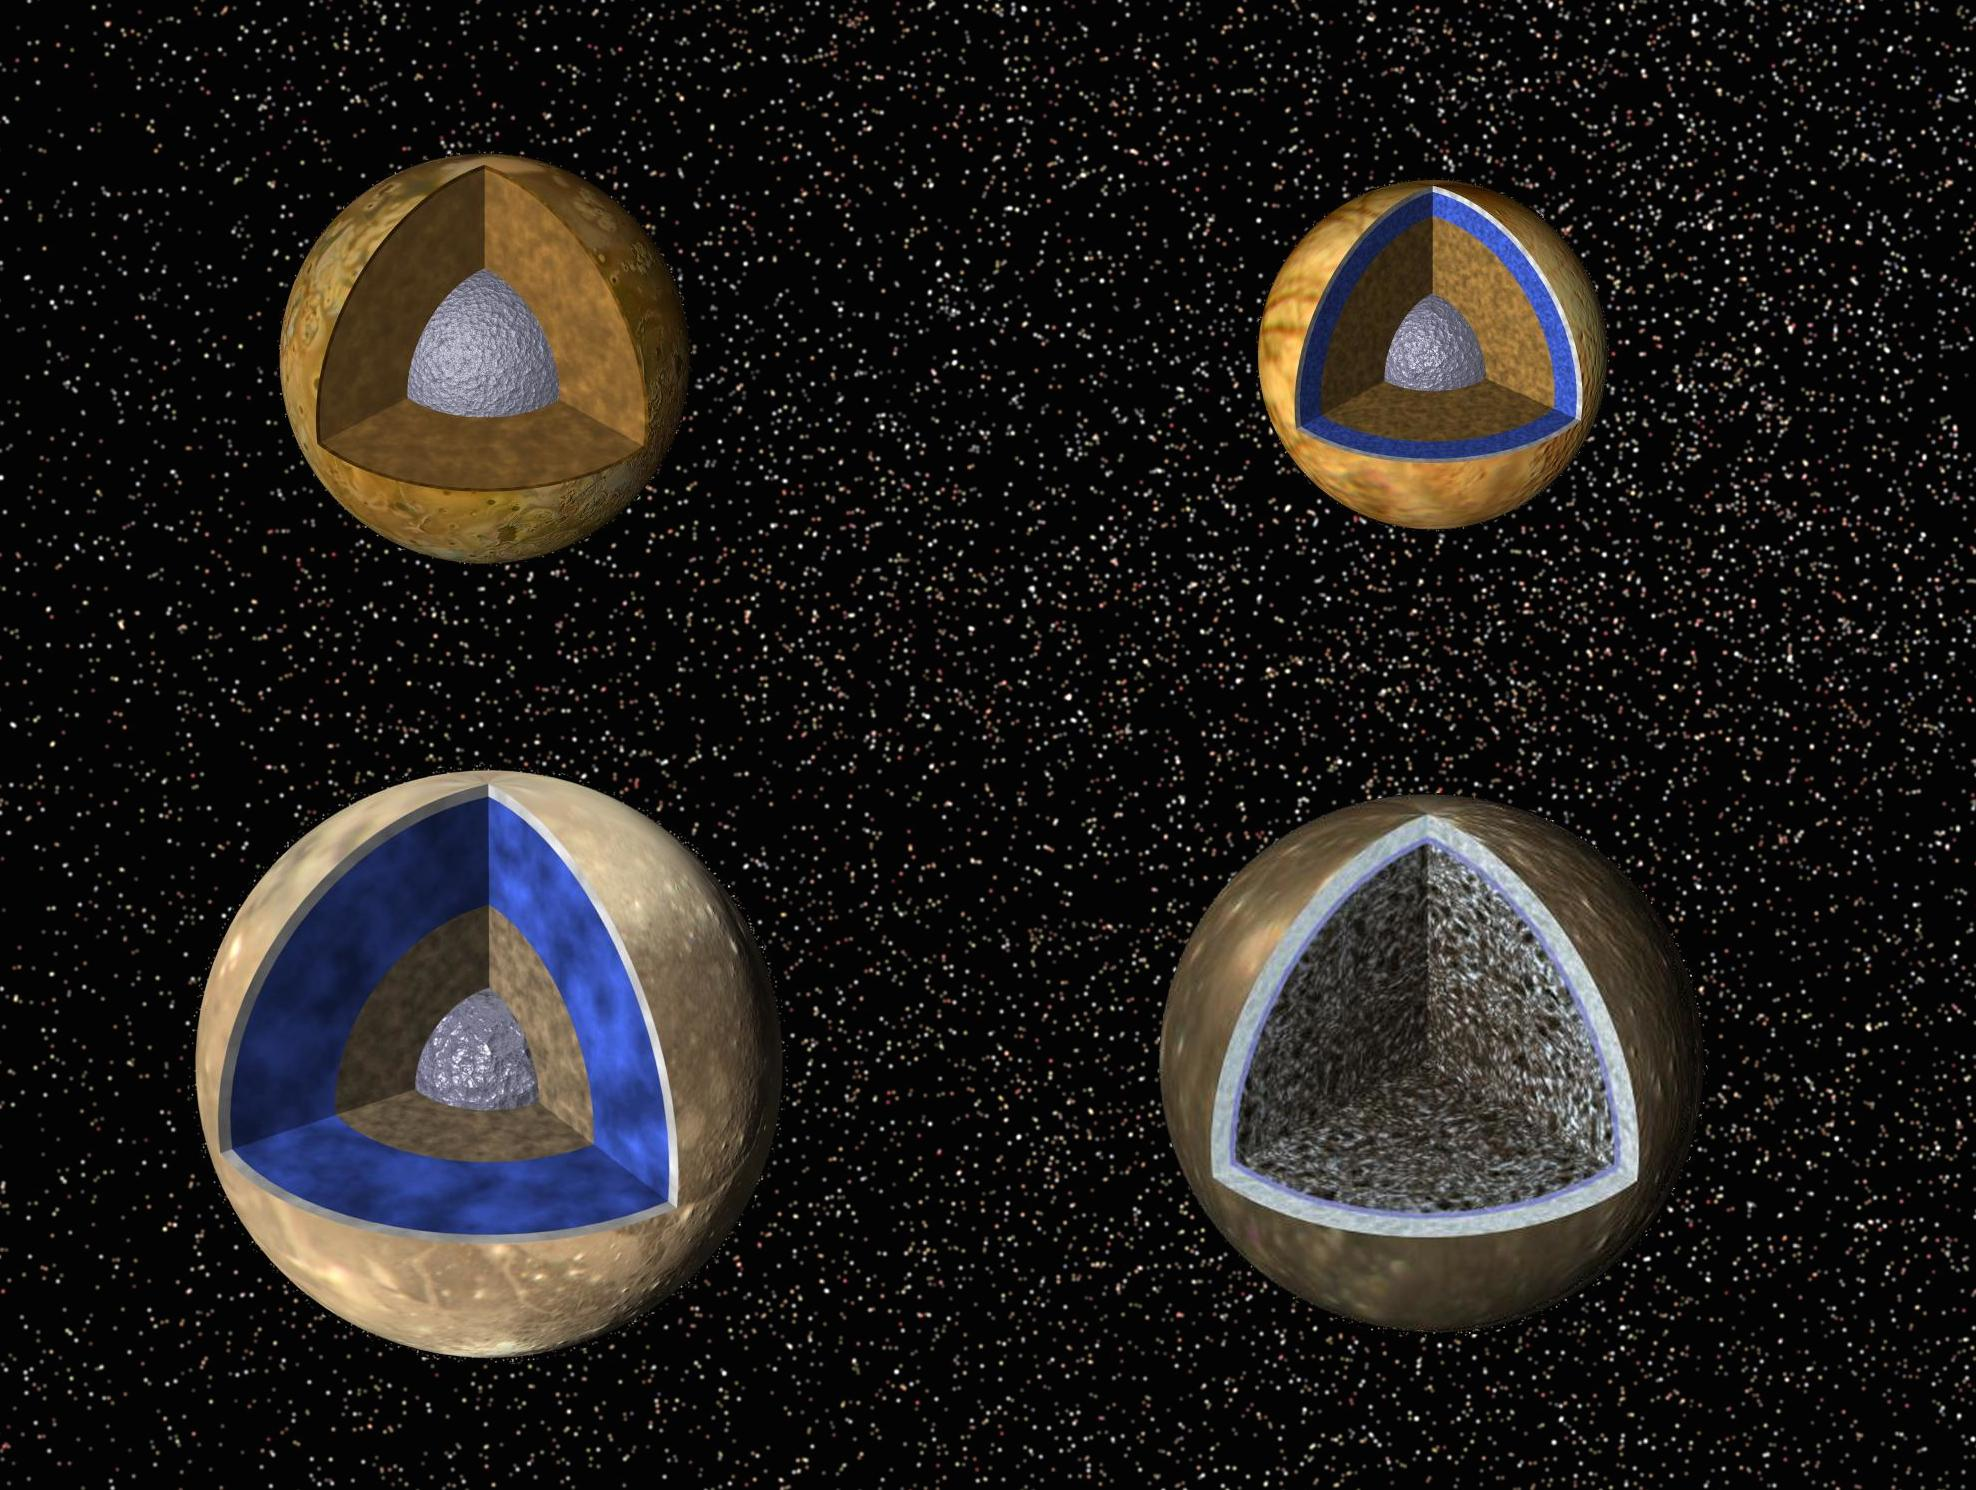
\includegraphics[width=\textwidth]{Galilean_sats_interiors}
	\caption{
	\scriptsize
	{\em Interiors of the Galilean Satellites}
	\label{galsats}
	}
\end{figure}
\end{center}
\end{textblock}

\end{document}
